\chapter{Analisi}
\label{chap:analisi}

\section{Analisi del problema}
\label{sec:analisi-problema}

Come anticipato nella Sezione~\ref{subsec:alchemist-osm}, il supporto geospaziale di
Alchemist consente di collocare e muovere con precisione i nodi di una simulazione su
cartografia reale, ma non offre un modo altrettanto maturo per esporre loro dati geospaziali,
in un dato istante, nel punto dello spazio geografico in cui si trovano.
L'interfaccia \texttt{Layer<T, P>} (Sezione~\ref{subsec:alchemist-layer}) è generica sia
nella posizione \texttt{P} sia nel valore \texttt{T} restituito, ma nessuna delle sue
implementazioni preesistenti espone dati che rappresentino misurazioni del mondo reale.

I dati geospaziali misurati, quali quelli distribuiti dai data store Copernicus descritti
nella Sezione~\ref{sec:copernicus}, differiscono dai valori sintetici prodotti dalle
implementazioni preesistenti per diversi aspetti:

\begin{itemize}
    \item sono distribuiti in un formato specialistico (\ac{NetCDF} o \ac{GRIB},
    Sezione~\ref{sec:formati-raster}), il cui schema (quali dimensioni compaiano, in quale
    ordine, con quale direzione degli assi, con quale nome interno la grandezza di interesse
    sia identificata) non è fissato a priori, ma varia da dataset a dataset;
    \item sono campionati su una griglia sia nello spazio sia nel tempo, mentre la
    posizione richiesta a un layer e l'istante di simulazione corrente sono entrambi
    quantità continue: fra un campione e l'altro non esiste, nel dato
    originale, alcun valore, e va quindi stabilita una regola per produrne uno;
    \item ciascuna griglia è riferita a un istante assoluto del mondo reale, espresso
    secondo un calendario, mentre il tempo di una simulazione Alchemist è un valore scalare
    privo di unità di misura intrinseca (Sezione~\ref{subsec:alchemist-time}), la cui
    interpretazione è una convenzione lasciata al modellista;
    \item non tutte le celle di una griglia riportano una misura: i formati prevedono un
    valore convenzionale per quelle che ne sono prive;
    \item non sono calcolabili localmente, vanno ottenuti da un
    servizio remoto che risponde in modo asincrono, secondo il paradigma descritto nella
    Sezione~\ref{sec:ogc-api-processes}, senza garanzia di completamento della richiesta.
\end{itemize}

Questi aspetti individuano i seguenti sotto-problemi:

\begin{enumerate}
    \item \textbf{Rappresentazione}: come rappresentare in memoria, in modo indipendente dalla fonte
    specifica del dato, una serie temporale di griglie raster geospaziali, le cui celle possono
    non ospitare una misurazione;
    \item \textbf{Risoluzione}: date una posizione geografica e un istante di simulazione
    arbitrari, come stabilire a quale istante del mondo reale essi corrispondano e come
    produrre un valore a partire da campioni discreti nello spazio e nel tempo, con
    possibili misurazioni mancanti;
    \item \textbf{Acquisizione}: come ottenere questi campioni da un servizio remoto asincrono, in modo
    riproducibile e verificabile, senza doverli riscaricare a ogni esecuzione della
    simulazione.
\end{enumerate}

\iffalse
I tre sotto-problemi sono debolmente accoppiati fra loro: la rappresentazione di una serie
di griglie è indipendente dalla loro provenienza, la risoluzione di un valore lo è dal modo
in cui le griglie sono state ottenute, e l'acquisizione lo è dal modo in cui i dati
acquisiti verranno successivamente letti. L'unico punto di contatto è la forma in cui i
dati vengono consegnati, ovvero un insieme di file in uno dei formati descritti nella
Sezione~\ref{sec:formati-raster}.
\fi

\section{Obiettivi}
\label{sec:obiettivi}

L'obiettivo generale del lavoro è dotare Alchemist della capacità di esporre ai nodi
di una simulazione grandezze geospaziali misurate, in funzione della posizione che essi
occupano e dell'istante di simulazione in cui vi accedono, ottenendole dai data store
Copernicus.

Per ogni sotto-problema individuato nella sezione precedente viene individuato
un sotto-obiettivo:

\begin{enumerate}
    \item \textbf{Rappresentazione}: definire una rappresentazione in memoria di una serie
    temporale di griglie raster geospaziali che sia indipendente dal formato e dalla fonte
    da cui i dati provengono, e che tenga conto sia dell'estensione spaziale e temporale
    entro la quale la grandezza è nota, sia dell'assenza di misura in alcune delle sue
    celle;

    \item \textbf{Risoluzione}: rendere tale rappresentazione interrogabile in una posizione
    geografica e a un istante di simulazione arbitrari. Ciò comprende lo stabilire quale
    istante del mondo reale corrisponda a un dato tempo di simulazione, e quale valore
    restituire quando la posizione e l'istante così individuati non coincidono con alcun
    campione disponibile; la regola con cui tale valore viene prodotto deve poter essere
    scelta in funzione della semantica della grandezza esposta, anziché essere fissata una
    volta per tutte;

    \item \textbf{Acquisizione}: dotare il simulatore della capacità di ottenere
    autonomamente dai data store Copernicus i dati necessari a una simulazione,
    conservandoli localmente in modo che esecuzioni successive che utilizzano gli stessi
    dati possano riutilizzarli.
\end{enumerate}

\iffalse
A questi si affianca un quesito preliminare. La proposta iniziale del lavoro ipotizzava che
l'interfaccia dei layer di Alchemist (Sezione~\ref{subsec:alchemist-layer}) dovesse essere
rivista per accogliere dati provenienti da fonti esterne. Stabilire se e in che misura ciò
sia necessario è parte dell'analisi, e ne condiziona il perimetro: la
Sezione~\ref{subsec:api-sufficiente} vi risponde una volta delimitati i requisiti.
\fi

Il risultato atteso è quindi un nuovo modulo del simulatore che aggiunga quanto descritto,
i cui componenti siano dichiarabili direttamente nella configurazione di una simulazione.

\section{Requisiti}
\label{sec:requisiti}

\subsection{Requisiti funzionali}
\label{subsec:requisiti-funzionali}

\begin{itemize}
    \item \textbf{F1 (Interrogazione spaziale)}: \label{req:F1} il modulo deve restituire
    un valore per una posizione geografica arbitraria interna all'estensione spaziale
    coperta dai dati.

    \item \textbf{F2 (Interrogazione temporale)}: \label{req:F2} il valore restituito deve
    essere quello percepito rispetto all'istante di simulazione corrente.

    \item \textbf{F3 (Corrispondenza temporale)}: \label{req:F3} la relazione fra il tempo
    di simulazione e gli istanti del mondo reale a cui i dati sono riferiti deve essere
    dichiarabile da chi conduce la simulazione, e non fissata dal modulo.

    \item \textbf{F4 (Risoluzione fra campioni)}: \label{req:F4} il modulo deve produrre un
    valore anche quando la posizione richiesta e l'istante individuato non coincidono con
    alcuno dei campioni disponibili.

    \item \textbf{F5 (Intercambiabilità della regola)}: \label{req:F5} la regola con cui
    tale valore viene prodotto deve poter essere scelta fra più alternative, senza
    richiedere modifiche al modulo.

    \item \textbf{F6 (Tipo esposto configurabile)}: \label{req:F6} il tipo del valore
    esposto ai nodi non deve coincidere necessariamente con quello numerico con cui la
    grandezza è registrata nel file, così da poter rappresentare anche grandezze la cui
    interpretazione non è puramente quantitativa.

    \item \textbf{F7 (Valori mancanti espliciti)}: \label{req:F7} le celle prive di misura
    presenti nei dati originali devono essere trattate in modo esplicito, e non ignorate o
    sostituite silenziosamente.

    \item \textbf{F8 (Indipendenza dal dataset)}: \label{req:F8} il modulo deve operare, con
    lo stesso codice, su più dataset e più data store Copernicus
    (Sezione~\ref{sec:copernicus}), senza conoscerne a priori lo schema.

    \item \textbf{F9 (Acquisizione autonoma)}: \label{req:F9} il modulo deve ottenere
    autonomamente i dati non ancora disponibili localmente e conservarli in una cache la
    cui posizione sia configurabile.

    \item \textbf{F10 (Riuso dei dati acquisiti)}: \label{req:F10} i dati già presenti in
    cache devono essere riutilizzati quando la configurazione della richiesta è invariata,
    senza effettuare nuove richieste di rete.

    \item \textbf{F11 (Configurazione dichiarativa)}: \label{req:F11} il modulo deve essere
    configurabile da un file YAML di simulazione (Sezione~\ref{subsec:alchemist-loader})
    senza richiedere obbligatoriamente la scrittura di codice; ciò vale anche per la scelta
    fra le alternative previste da \req{F5}.
\end{itemize}

\subsection{Requisiti non funzionali}
\label{subsec:requisiti-non-funzionali}

\begin{itemize}
    \item \textbf{NF1 (Additività)}: \label{req:NF1} il modulo deve realizzarsi come
    estensione del simulatore, senza richiedere modifiche al suo motore né alle astrazioni
    del suo modello.

    \item \textbf{NF2 (Genericità)}: \label{req:NF2} la parte che sa leggere e risolvere una
    serie temporale di griglie raster deve restare separata da quella che sa ottenerle dai
    data store Copernicus, così che la prima resti utilizzabile anche con fonti diverse da
    quelle qui considerate.

    \item \textbf{NF3 (Aderenza alle convenzioni di Alchemist)}: \label{req:NF3} il codice è
    destinato a una pull request verso il repository del simulatore, e deve quindi
    rispettarne le convenzioni di stile, di collocazione dei package e di configurazione
    degli strumenti di analisi statica.

    \item \textbf{NF4 (Testabilità senza rete)}: \label{req:NF4} nessun test deve dipendere
    dalla disponibilità dei data store Copernicus o dal possesso di credenziali valide.

    \item \textbf{NF5 (Riproducibilità)}: \label{req:NF5} la stessa richiesta verso un data
    store deve corrispondere in modo deterministico alla stessa voce di cache.

    \item \textbf{NF6 (Fallimento esplicito)}: \label{req:NF6} nessuna condizione anomala
    deve produrre un valore silenziosamente scorretto: deve produrre un errore con un
    messaggio diagnostico.

    \item \textbf{NF7 (Fallimento anticipato)}: \label{req:NF7} le condizioni che
    impediscono a una simulazione di disporre dei dati di cui ha bisogno devono
    manifestarsi al caricamento della simulazione, e non durante l'esecuzione.

    \item \textbf{NF8 (Costo dell'interrogazione)}: \label{req:NF8} il valore di un layer
    viene richiesto potenzialmente molte volte per ogni evento della simulazione: la lettura
    non deve comportare accessi a risorse esterne, e il suo costo non deve dipendere dalla
    provenienza dei dati.

    \item \textbf{NF9 (Uso concorrente della cache)}: \label{req:NF9} Alchemist consente
    l'esecuzione simultanea di più simulazioni; più esecuzioni che condividano la stessa
    cache e richiedano gli stessi dati non devono interferire fra loro, né produrre voci di
    cache incomplete o corrotte.
\end{itemize}

\section{Analisi dei requisiti}
\label{sec:analisi-requisiti}

Alcuni dei requisiti elencati richiedono un ragionamento preliminare, o pongono condizioni
la cui portata va delimitata prima di poter essere tradotte in scelte progettuali.

\subsection{La corrispondenza fra i domini temporali}
\label{subsec:corrispondenza-temporale}

Il requisito \req{F3} chiede di mettere in relazione due domini temporali di natura
diversa: gli istanti assoluti del mondo reale a cui i dati sono riferiti e il tempo
scalare della simulazione. La relazione può essere stabilita in due modi opposti:
eliminando la differenza alla radice, ovvero sostituendo il tipo di tempo del simulatore
con uno che rappresenti già un istante assoluto, oppure mantenendo il tipo esistente e
stabilendo una corrispondenza esplicita, confinandola nel componente che ne ha bisogno.

La prima strada è stata oggetto di uno studio di fattibilità, condotto sul codice del
simulatore con l'obiettivo di stimare l'estensione dell'intervento piuttosto che di
portarlo a termine.

L'ostacolo principale è di natura semantica. \texttt{Time} è oggi usato
indifferentemente per denotare un istante della simulazione e un intervallo fra due
istanti distinti: le due nozioni condividono lo stesso tipo e sono combinabili fra loro
tramite operazioni aritmetiche. Le astrazioni di \texttt{kotlin.time} le distinguono
invece in due tipi separati, \texttt{Instant} e \texttt{Duration}, fra i quali solo alcune
combinazioni sono ammesse: ad esempio, non è possibile moltiplicare un istante per uno
scalare. Allo stesso modo non si ha consistenza nel tipo di ritorno delle operazioni,
ad esempio sottrarre un \texttt{Instant} da un altro produce un \texttt{Duration}, mentre
\texttt{Time} ammette tutte queste operazioni e il loro risultato è sempre del medesimo
tipo. La sostituzione non è quindi meccanica: richiede di stabilire, per ogni punto d'uso,
quale dei due ruoli vi sia svolto, e la modifica di una firma si propaga a tutti i suoi
utilizzatori.

Un intervento di questa natura ricade sul motore del simulatore e sulle astrazioni del suo
modello, ed è quindi incompatibile con \req{NF1}. Si è pertanto scelto di percorrere la
seconda strada: mantenere inalterato il tipo di tempo del simulatore e stabilire la
corrispondenza fra i due domini nel solo componente che ne ha bisogno, dichiarata da chi
configura la simulazione come \req{F3} richiede.

\subsection{La discretezza dei campioni}
\label{subsec:discretezza-campioni}

Risolta la corrispondenza temporale, resta il problema posto da \req{F4}: quale valore
restituire quando l'istante richiesto cade fra due istanti campionati; formalmente, quale
valore restituire quando a ogni istante $t_{i}$ è associata una griglia spaziale e si ha
che il tempo di simulazione corrente $t_s \in [t_i, t_{i+1}]$, \Cref{fig:temp-interp}.

\begin{figure}[H]
    \centering
    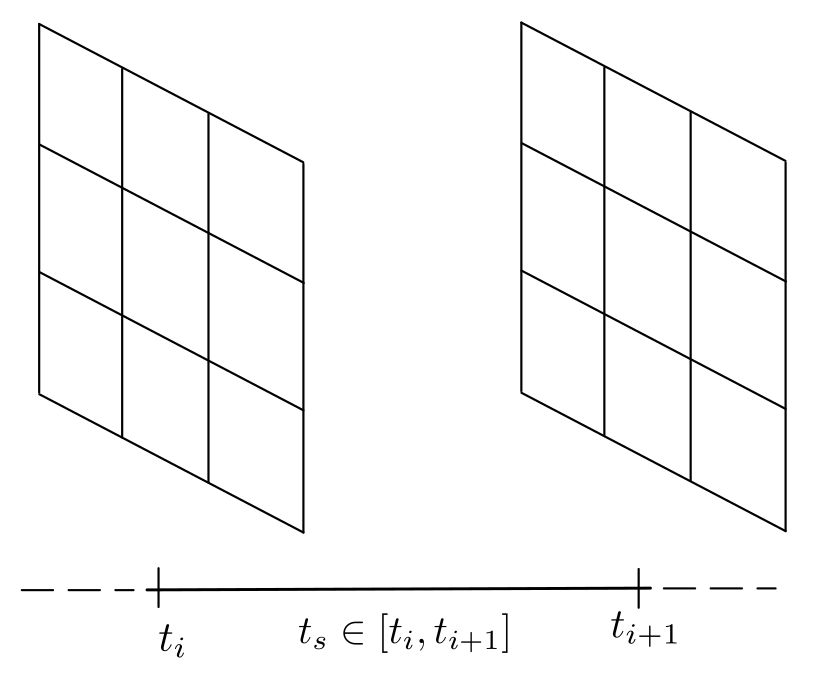
\includegraphics[width=0.6\linewidth]{figures/temporal_interpolation.png}
    \caption[Composizione temporale dei campioni]{L'istante identificato ricade nell'intervallo di due campionamenti.}
    \label{fig:temp-interp}
\end{figure}

E in modo del tutto analogo,
quando la posizione richiesta cade fra le celle della griglia spaziale; formalmente,
quale valore restituire per la posizione $P = (\text{lat}_{a}, \text{lon}_{b})$ quando
$\text{lat}_{a} \in [\text{lat}_{i}, \text{lat}_{i+1}]$ e $\text{lon}_{b} \in [\text{lon}_{j}, \text{lon}_{j+1}]$
, \Cref{fig:spatial-interp}.

\begin{figure}[H]
    \centering
    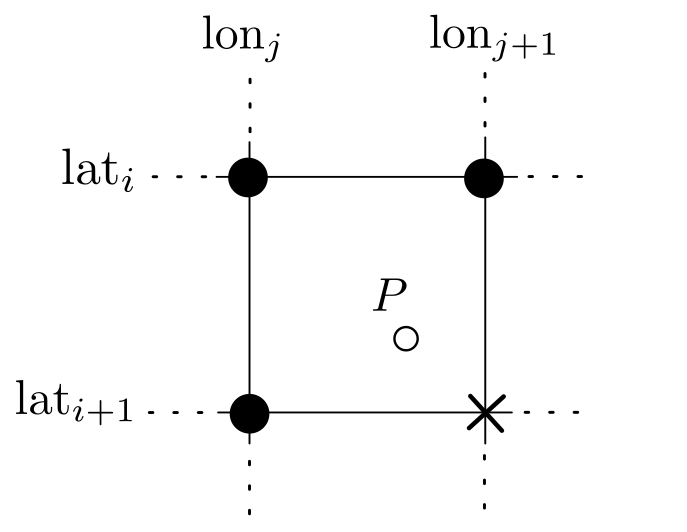
\includegraphics[width=0.5\linewidth]{figures/spatial_interpolation.png}
    \caption[Composizione spaziale dei campioni]{La posizione richiesta ricade tra le misurazioni. I cerchi pieni rappresentano misurazioni disponibili,
    la croce rappresenta una misurazione assente.}
    \label{fig:spatial-interp}
\end{figure}

La risposta richiede una regola di combinazione dei campioni adiacenti, e tale regola non
può essere unica. Una grandezza che varia con continuità, come la temperatura, ammette
naturalmente una combinazione pesata dei campioni che la circondano; al contrario, un dato
di natura categorica (come il codice convenzionale che distingue pioggia, neve o grandine)
non ammette interpolazioni intermedie: tali grandezze richiedono di selezionare un singolo
campione secondo un criterio esplicito, ad esempio il campione spazialmente più vicino.
La scelta dipende dalla semantica del dato, non dal meccanismo che lo espone, e non può
quindi essere fissata una volta per tutte nel codice del modulo.

È questa osservazione a motivare \req{F5}: la regola con cui un valore viene prodotto a
partire dai campioni disponibili, sia temporali sia spaziali, deve essere configurabile e
intercambiabile.

La stessa regola è inoltre il punto in cui si decide come comportarsi con le celle prive di
misura, di cui \req{F7} chiede un trattamento esplicito: se una posizione richiesta è
circondata anche da un solo campione assente, non esiste una risposta valida per ogni
grandezza, e la decisione se propagare l'assenza, ignorarla o convertirla ricade nuovamente
sulla semantica del dato.

\subsection{Il dominio di definizione del layer}
\label{subsec:estensione-spaziale}

I requisiti \req{F1} e \req{F2} sono formulati su una posizione geografica e un istante di
simulazione arbitrari: va stabilito entro quali confini tale arbitrarietà sia ammissibile.

Sul dominio spaziale, ogni dataset copre una regione geografica delimitata, e una posizione
esterna a essa non corrisponde ad alcuna misura. Produrre comunque un valore, ad esempio
riportando la posizione al bordo della copertura, significherebbe restituire un numero
plausibile ma privo di fondamento nei dati, tanto più fuorviante quanto più la posizione
richiesta è lontana dalla regione coperta; ciò contrasterebbe con \req{NF6}, che vieta la
produzione di valori silenziosamente scorretti. Il layer è quindi definito sulla sola
estensione spaziale dei dati che espone, e una richiesta al di fuori di essa è da
considerarsi un errore di modellazione della simulazione, da segnalare come tale.

La delimitazione è sostenibile perché l'estensione spaziale è nota prima
dell'esecuzione: essa coincide con l'area richiesta al data store, e la collocazione
dei nodi e i percorsi lungo i quali essi si muovono ricadono su chi configura
la simulazione. Una posizione esterna è quindi data da un'incoerenza fra i
dati richiesti e l'ambiente simulato.

\iffalse
Sul dominio temporale la situazione è diversa. Il tempo di simulazione può avanzare
indefinitamente a partire dallo zero. Rifiutare la richiesta, come sul dominio
spaziale, significherebbe interrompere una simulazione altrimenti valida. Il layer resta
quindi definito sull'intero asse temporale, e la regola con cui produce un valore al di
fuori dell'intervallo coperto è discussa nel Capitolo~\ref{chap:progettazione}.
\fi

Sul dominio temporale la situazione è diversa. Il tempo di una simulazione avanza
indefinitamente a partire dallo zero, e il momento in cui essa termina non è
necessariamente noto a chi la configura. Alchemist consente di dichiarare condizioni
di terminazione, verificate dopo ogni evento, ma non ne richiede per forza una.

Ne consegue che una limitazione sul dominio temporale avrebbe una portata diversa da
quello sul dominio spaziale. Sul dominio spaziale il rifiuto segnala un'incoerenza
fra i dati richiesti e l'ambiente simulato, per la quale nessuna risposta sarebbe
corretta. Sul dominio temporale interromperebbe invece una simulazione potenzialmente
coerente.

Il layer resta quindi definito sull'intero asse temporale, e la regola con cui
produce un valore al di fuori dell'intervallo coperto è discussa nella
Sezione~\ref{sec:corrispondenza-temporale}.

\subsection{Le ipotesi sui dati utilizzati}
\label{subsec:griglie-supportate}

Il requisito \req{F8} chiede che il modulo operi, con lo stesso codice, su dataset diversi
senza conoscerne a priori lo schema. Perché ciò sia possibile occorre stabilire che cosa
tali dataset debbano avere in comune, ovvero quali proprietà siano date per acquisite
sui dati di ingresso.

Due discendono direttamente da ciò che il layer espone. La prima è che la grandezza di
interesse dipenda dalle sole tre dimensioni tempo, latitudine e longitudine: sono le sole
rispetto alle quali il layer viene interrogato (\req{F1}, \req{F2}), e un dataset definito
anche su altre dimensioni, come la quota o il livello di pressione, non individuerebbe un
valore unico per una posizione e un istante. La seconda è che i file che descrivano una
stessa serie condividano la medesima griglia e la medesima grandezza, ovvero l'omogeneità
che la Sezione~\ref{sec:modello-dominio} attribuisce a una serie di griglie.

La terza è invece una restrizione effettiva del campo di applicabilità: si assume che la
griglia spaziale sia definita da un asse di latitudini e uno di longitudini indipendenti e
strettamente monotoni, non necessariamente a passo costante. Come osservato nella
Sezione~\ref{sec:formati-raster}, non tutti i dataset distribuiti dai data store la
soddisfano: alcuni sono campionati su una griglia nativa in una proiezione cartografica,
nella quale le coordinate geografiche di ciascuna cella sono note ma non ottenibili come
prodotto cartesiano di due assi indipendenti. Individuare la cella che contiene una data
posizione richiede allora di invertire la proiezione fra il sistema di riferimento del
dataset e quello geografico.

La restrizione è stata ritenuta accettabile perché la forma di distribuzione
prevalente prevede una griglia in latitudine e longitudine, sulla quale il
servizio consente di ritagliare l'area geografica di interesse al momento della richiesta.

Sul dominio temporale non viene invece posta alcuna ipotesi oltre alla distinzione e
all'ordinamento degli istanti: l'ampiezza degli intervalli che li separano può variare
liberamente lungo la serie.

\subsection{Il momento del fallimento}
\label{subsec:momento-del-fallimento}

L'acquisizione dei dati da un servizio remoto, richiesta da \req{F9}, è l'unica parte del
lavoro soggetta a condizioni fuori dal controllo del modulo: la rete può non essere
disponibile, le credenziali possono mancare o essere scadute, il servizio può rifiutare la
richiesta o consegnare dati incompleti.

Il requisito \req{NF7} stabilisce che tutte queste condizioni si manifestino al momento del
caricamento della simulazione: una simulazione parte solo se dispone di tutti i dati di
cui ha bisogno, altrimenti non parte affatto, segnalando il motivo.

La scelta garantisce una proprietà utile a chi conduce esperimenti: il fallimento è
immediato e riconoscibile, anziché manifestarsi a esecuzione avanzata sotto forma di
risultati alterati.

\subsection{L'adeguatezza dell'interfaccia dei layer}
\label{subsec:api-sufficiente}

La revisione dell'interfaccia dei layer era fra le ipotesi di partenza
del progetto: \texttt{Layer<T,P>} è stata concepita per grandezze calcolabili
localmente, ed è lecito chiedersi se sia adeguata ad accogliere dati misurati
provenienti da fonti esterne. Delimitati i requisiti, la domanda viene affrontata
verificando quali fra essi pongano condizioni sulla forma dell'interrogazione
anziché sul modo in cui il valore viene prodotto.

Nessuno fra i requisiti funzionali riguarda la forma con cui il valore viene richiesto:
tutti riguardano il modo in cui esso viene prodotto. In particolare, \req{F1}, \req{F2} e \req{F4} pongono
condizioni sul valore restituito da un'interrogazione la cui firma resta quella esistente;
\req{F3} riguarda una corrispondenza fissata alla costruzione del layer;
\req{F5}, \req{F6} e \req{F7} riguardano componenti interni al layer; \req{F8}, \req{F9} e
\req{F10} riguardano l'origine dei dati, che il layer riceve già costruiti; \req{F11}
riguarda il meccanismo di caricamento, esterno all'interfaccia.

Resta una sola limitazione, ed è di natura diversa. Il valore restituito da un layer che
espone dati misurati può, in linea di principio, cambiare in due modi distinti: perché il
tempo di simulazione avanza e il layer legge un istante diverso di una serie di dati già
disponibile, oppure perché il dato sottostante viene aggiornato dall'esterno durante
l'esecuzione. Il primo caso è quello descritto da \req{F2}, e non pone alcun problema
all'interfaccia esistente: la lettura resta funzione della sola posizione richiesta e del
tempo di simulazione corrente. Il secondo richiederebbe invece un layer mutabile durante
l'esecuzione, il quale è a sua volta subordinato a una revisione del motore reattivo di
Alchemist non ancora disponibile.

\iffalse
Di conseguenza la serie di dati esposta dal layer è fissata al momento della costruzione
e non muta per l'intera durata della simulazione. Con questa delimitazione, e una volta
separate la lettura dei dati, la regola di combinazione dei campioni e la loro
acquisizione, l'interfaccia esistente si è rivelata adeguata così com'è.

Ne consegue che \req{NF1} è soddisfacibile: il lavoro qui descritto è puramente additivo
rispetto al simulatore, e si realizza come un nuovo modulo che implementa un'interfaccia
esistente, senza richiedere modifiche al motore né alle astrazioni del suo modello.
\fi

Con questa delimitazione, e una volta separate la lettura dei dati, la regola
di combinazione dei campioni e la loro acquisizione, l'interfaccia esistente si è
rivelata adeguata così com'è. Di conseguenza \req{NF1} è rispettabile: il lavoro qui descritto
è puramente additivo rispetto al simulatore, e si realizza come un nuovo modulo che implementa
un'interfaccia esistente.

\section{Modello del dominio}
\label{sec:modello-dominio}

Questa sezione individua le entità in gioco e le relazioni che le legano; la
\Cref{fig:modello-dominio} le riporta. Il modello si limita alle astrazioni: le loro
realizzazioni concrete e il modo in cui vengono composte fra loro sono presentate nel
Capitolo~\ref{chap:progettazione}. Per ciascuna entità sono indicati i requisiti a cui
essa risponde.

\begin{figure}[H]
    \centering
    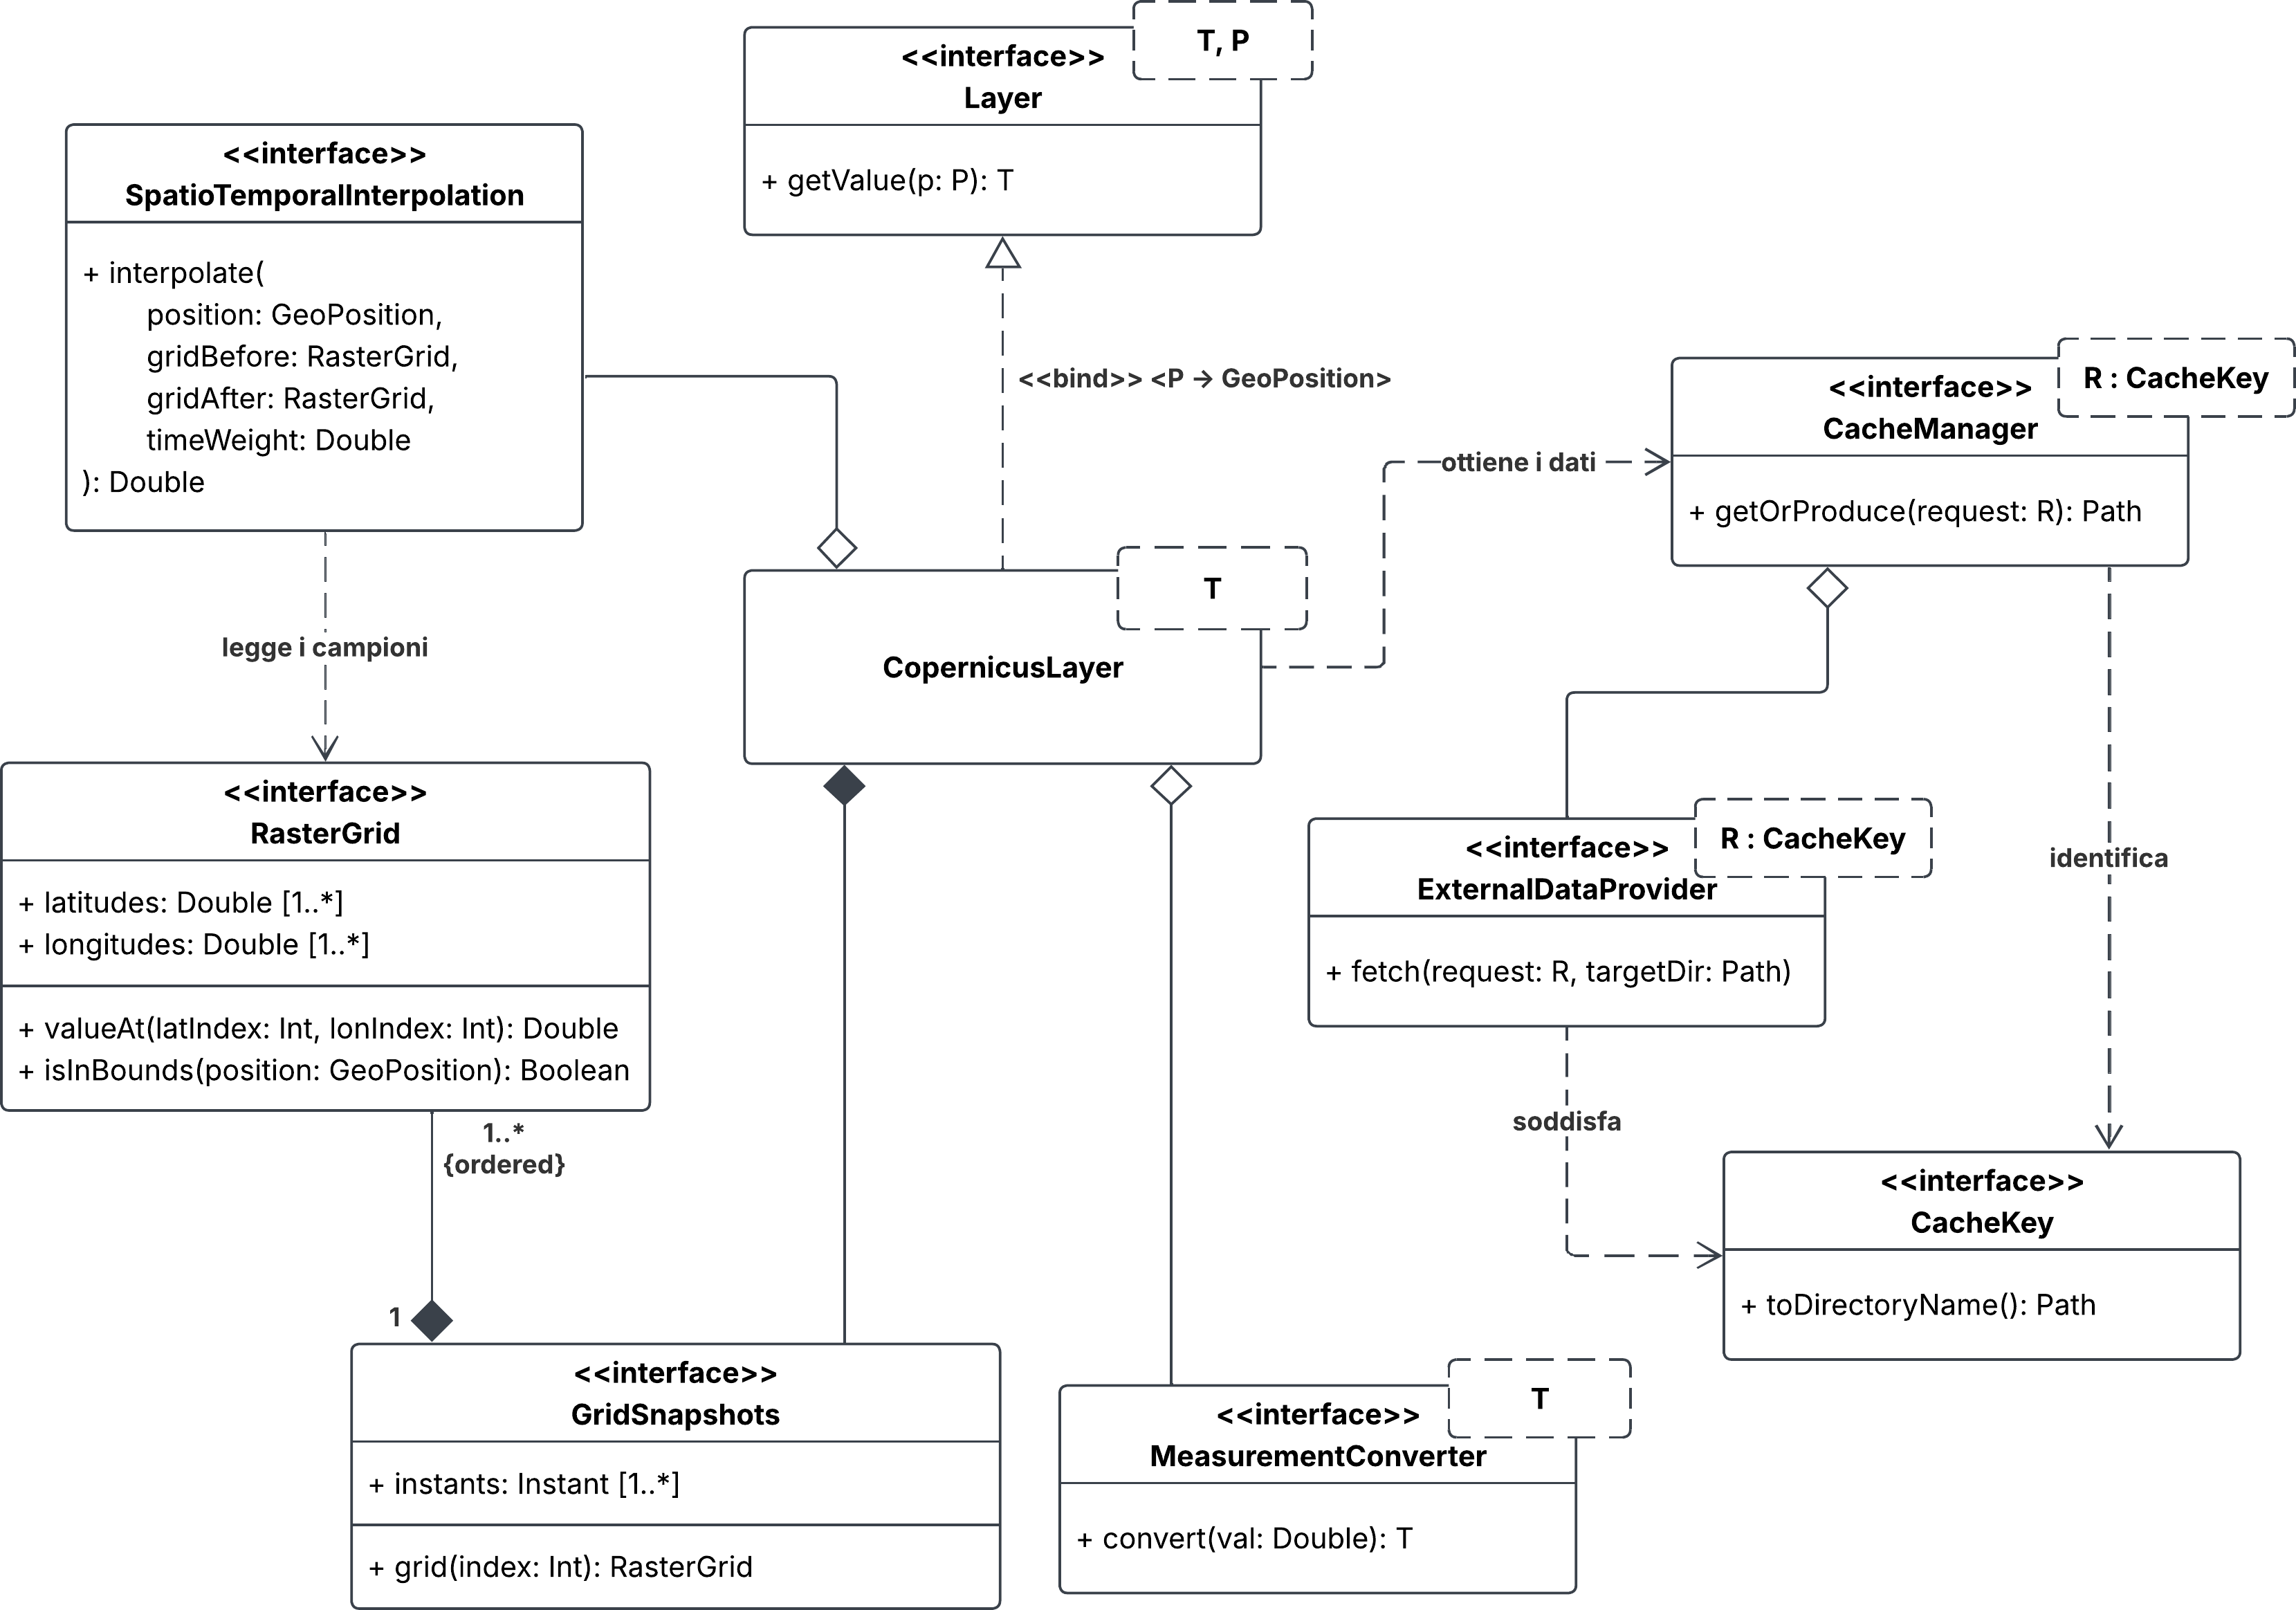
\includegraphics[width=\linewidth]{figures/uml_dominio.png}
    \caption[Modello del dominio]{Le entità del dominio e le relazioni fra di esse.}
    \label{fig:modello-dominio}
\end{figure}

\begin{itemize}
    \item \texttt{RasterGrid} (\req{F1}, \req{F7}, \req{F8}): l'insieme dei campioni di una
    grandezza relativi a un singolo istante, organizzati su un reticolo definito da un asse
    di latitudini e uno di longitudini indipendenti e strettamente monotoni, secondo
    l'ipotesi stabilita nella Sezione~\ref{subsec:griglie-supportate}. Questa griglia
    delimita l'estensione spaziale entro la quale la grandezza è nota, e le sue celle
    possono non ospitare alcuna misura.

    \item \texttt{GridSnapshots} (\req{F2}, \req{F4}, \req{F8}): una successione di griglie
    fra loro omogenee, ovvero relative alla stessa grandezza e agli stessi assi spaziali,
    ciascuna associata a un istante del mondo reale distinto dagli altri. Gli istanti sono
    ordinati, ma non necessariamente equispaziati, e delimitano l'estensione temporale
    entro la quale la grandezza è nota.

    \item \texttt{CopernicusLayer} (\req{F1}, \req{F2}, \req{F3}): la realizzazione di un
    \texttt{Layer} su posizioni geografiche (\texttt{GeoPosition}) che espone una serie di
    griglie. Stabilisce fra il tempo di simulazione e quello del mondo reale la
    corrispondenza discussa nella Sezione~\ref{subsec:corrispondenza-temporale}, e
    individua i campioni pertinenti all'istante in cui viene interrogato.

    \item \texttt{SpatioTemporalInterpolation} (\req{F4}, \req{F5}): la regola con cui,
    dalle due griglie adiacenti all'istante richiesto e dai campioni che circondano la
    posizione richiesta, si ottiene un valore per quella posizione e quell'istante. La
    regola attraversa entrambi i domini, spaziale e temporale, ed è per questo espressa da
    un'unica astrazione. La sua scelta dipende dalla semantica della grandezza esposta.

    \item \texttt{MeasurementConverter} (\req{F6}, \req{F7}): il criterio con cui il valore
    numerico prodotto dalla regola di risoluzione viene tradotto nel valore esposto dal
    layer, compreso il caso in cui i campioni necessari a produrlo siano assenti. È ciò che
    consente al layer di esporre anche grandezze la cui interpretazione non è quantitativa.

    \item \texttt{CacheKey} (\req{F10}, \req{NF5}): la descrizione dei dati da ottenere da
    una fonte esterna. Ne costituisce l'identità, nel senso che due descrizioni uguali
    individuano gli stessi dati: è questo a rendere possibile riconoscere se sono già stati
    ottenuti in precedenza e quindi individuabili in cache.

    \item \texttt{ExternalDataProvider} (\req{F9}, \req{NF2}): la fonte in grado di
    soddisfare una descrizione, consegnando i dati corrispondenti in forma di file.

    \item \texttt{CacheManager} (\req{F9}, \req{F10}, \req{NF9}): l'entità che, data una
    descrizione, restituisce i dati corrispondenti, interpellando la fonte esterna solo
    quando questi non siano già disponibili localmente.
\end{itemize}

Le entità si dispongono lungo i tre sotto-problemi individuati nella
Sezione~\ref{sec:analisi-problema}. Le prime due riguardano la rappresentazione, le tre
successive la risoluzione di un valore, le ultime tre l'acquisizione. Ogni requisito
funzionale è coperto da almeno un'entità, a eccezione di \req{F11}, che non riguarda le
entità del dominio bensì il modo in cui esse vengono rese dichiarabili nella
configurazione di una simulazione.

\iffalse
Le uniche relazioni che attraversano i confini fra un gruppo e l'altro sono due: quella
fra il layer e la serie di griglie che espone, e quella fra il layer e il gestore della
cache dal quale ottiene i dati da cui la serie viene costruita. Nessuna entità dell'area di
acquisizione compare fra quelle di cui il layer ha bisogno per restituire un valore, coerentemente con \req{NF8}.
\fi

Le relazioni che attraversano i confini fra un gruppo e l'altro sono tre: quella fra
il layer e la serie di griglie che espone, quella fra la regola di risoluzione e le griglie
sulle quali essa opera, e quella fra il layer e il gestore della cache dal quale ottiene
i dati da cui la serie viene costruita.